\documentclass[border=10pt]{standalone}
\usepackage{pgfplots}
\pgfplotsset{compat=1.18}
\usetikzlibrary{arrows.meta} % Explicitly load library for arrow tips
\usepackage{amsmath,amssymb,amsthm}

\begin{document}
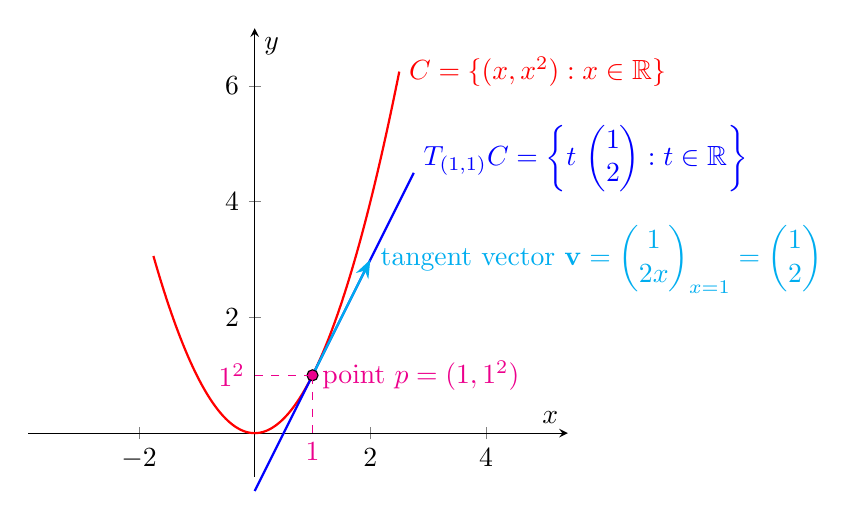
\begin{tikzpicture}
% --- Pre-calculate all values for maximum robustness ---
\pgfmathsetmacro{\a}{1}          % x-coordinate of point p
\pgfmathsetmacro{\ay}{\a^2}        % y-coordinate of point p
\pgfmathsetmacro{\slope}{2*\a}     % Slope (derivative) at p
\pgfmathsetmacro{\dx}{1}           % Vector x-component
\pgfmathsetmacro{\dy}{\slope * \dx} % Vector y-component
\pgfmathsetmacro{\endx}{\a + \dx}   % Vector end-point x
\pgfmathsetmacro{\endy}{\ay + \dy}   % Vector end-point y
\pgfmathsetmacro{\labelx}{3}       % x-pos for the T_pC label
\pgfmathsetmacro{\labely}{\ay+\slope*(\labelx-\a)} % y-pos for the T_pC label

\begin{axis}[
	axis lines=center,
	xlabel=$x$,
	ylabel=$y$,
	legend pos=north west,
	xmin=-.5, xmax=2,
	ymin=-.75, ymax=7,
	axis equal, % Ensures slopes are visually correct
	clip=false,
	]
	
	% --- Plot the curve y=x^2 ---
	\addplot[domain=-1.75:2.5, samples=100, thick, red] {x^2};
	%	\addlegendentry{$C: y=x^2$};
	\node[right, red] at (axis cs: 2.5, {2.5^2}) {$C=\{(x,x^2):x\in\mathbb{R}\}$};
	
	% --- Plot the tangent line at x=a ---
	\addplot[domain=0:2.75, samples=2, thick, blue] {\ay + \slope*(x-\a)};
	\node[right, blue] at (axis cs: 2.75, 4.75) {$T_{(1,1)}C=\left\{t\,\begin{pmatrix} 1 \\ 2 \end{pmatrix}:t\in\mathbb{R}\right\}$};
	
% Use pre-calculated coordinates for the label
%	\node[above, rotate=atan(\slope), black!60] at (axis cs: \labelx, \labely) {$T_pC$};
%	

	% --- Draw the tangent vector v=<dx,dy> ---
	\draw[
	-{Stealth}, % Arrow tip from arrows.meta library
	thick,
	cyan,
	] (axis cs: \a, \ay) -- (axis cs: \endx, \endy)
	node[right] {tangent vector $\mathbf{v} = \begin{pmatrix}
			1 \\ 2x
		\end{pmatrix}_{x=1}= \begin{pmatrix} 1 \\ 2 \end{pmatrix}$};	
%	\draw[dashed, cyan] (1,3) node[above] {$1$} -- (2,3);
%	\draw[dashed, cyan] (\a,\ay) to (0,\ay) node[left] {$1^2$};
	
		% --- Mark the point p ---
	%	\node[circle, fill=magenta, inner sep=1.5pt, label={right:$p=(a, a^2)$}] at (axis cs: \a, \ay) {};
	\draw[fill=magenta] (\a, \ay) circle (2pt) node[right, magenta] {point $p=(1, 1^2)$};
	\draw[dashed, magenta] (\a,\ay) to (\a,0) node[below] {$1$};
	\draw[dashed, magenta] (\a,\ay) to (0,\ay) node[left] {$1^2$};
\end{axis}
\end{tikzpicture}
\end{document}